% \appendix
\renewcommand{\thechapter}{A}
\chapter{Usage of AlgTest pyProcess}

\definecolor{codegreen}{rgb}{0,0.6,0}
\definecolor{codegray}{rgb}{0.5,0.5,0.5}
\definecolor{codepurple}{rgb}{0.58,0,0.82}
\definecolor{backcolour}{rgb}{0.95,0.95,0.92}

\lstdefinestyle{mystyle}{
    backgroundcolor=\color{white},   
    commentstyle=\color{codegreen},
    keywordstyle=\color{magenta},
    numberstyle=\tiny\color{codegray},
    stringstyle=\color{codepurple},
    basicstyle=\ttfamily\footnotesize,
    breakatwhitespace=false,         
    breaklines=true,                 
    captionpos=b,                    
    keepspaces=true,                          
    showspaces=false,                
    showstringspaces=false,
    showtabs=false,                  
    tabsize=2
}

\lstset{style=mystyle}

\section{Installation}
After cloning into the repository containing \texttt{AlgTest process} tool, it is necessary to install a few dependencies. The project includes a script called \texttt{setup.py} which, when ran installs required packages. It may be convenient to create a Python virtual environment that allows us to install and manage Python project packages locally without unnecessary global installation. It is important to create and source a virtual environment before running the setup script.
\begin{lstlisting}[language=bash]
    $ python -m venv venv
    $ source venv/bin/activate
    $ python setup.py
\end{lstlisting}

\section{Folder structure}
\begin{itemize}
    \item \texttt{algtestprocess}
        \begin{itemize}
            \item \texttt{modules} -- folder containing \texttt{algtestprocess} modules.
                \begin{itemize}
                    \item \texttt{components} -- folder containing reusable code for parts of HTML documents. Each file contains classes, constants related to one component.
                    \item \texttt{pages} -- folder containing files with classes corresponding to generated HTML pages, each page has a separate file containing classes that are responsible for page creation.
                    \item \texttt{visualization} -- folder containing specific standalone visualizations which can be used independently or as a part of created pages.
                    \item \texttt{parser}
                        \begin{itemize}
                            \item \texttt{javacard} -- folder containing parser implementations for JavaCard profiles
                            \item \texttt{tpm} -- folder containing parser implementations for TPM profiles
                        \end{itemize}
                    \item \texttt{config.py} -- file containing classes for choice of algorithms used in specific pages
                    \item \texttt{jcalgtest.py} -- file containing classes for storage of Java Card device profiles
                    \item \texttt{tpmalgtest.py} -- file containing classes for storage of TPM device profiles
                \end{itemize}
        \end{itemize}
    \item \texttt{assets} -- folder which contains CSS and JavaScript assets that are used in visualizations, the folder was created from CSS and JavaScript assets which were used by \texttt{JCAlgTest process}.
    \item \texttt{setup.py} -- script for installation of dependencies and download of results from their official GitHub repository\footnote{\url{https://github.com/crocs-muni/jcalgtest_results}}, which is an official repository for JavaCard datasets, but also contains some TPM datasets. This repository at the time of writing contains only a subset of tested TPMs with no cryptographic properties. Complete datasets for TPMs are not publicly available for now. 
    \item \texttt{process.py} -- main entry point for the generation of outputs, its usage is described in the following section
\end{itemize}

\section{Usage}
The script process.py provides following CLI arguments and options:

\begin{itemize}
    \item Device type which is either \texttt{tpm} or \texttt{javacard}.
    \item Set of operations from \texttt{process, all, execution-time, comparative, radar, scalability, similarity, support, compare, and heatmap}. All of them except for the special operations \texttt{process} and \texttt{all} signify a type of visualization.
    
    A set of operations can be selected, but when generating visualizations for JavaCards, then a \texttt{process} operation needs to be run at least once so that some issues with CSV files are fixed, and JSON outputs are generated for the following operations which use them. In the subsequent runs the \texttt{process} argument is not necessary.
    
    The \texttt{all} operation tells the script to generate all possible visualizations for a given device.
    \item \texttt{-i/-{}-results-dir} A directory with device profiles. It is important that profiles of only one device type are contained in the children directories.
    \item \texttt{-o/-{}-output-dir} Output directory to which the HTML outputs are stored. 
\end{itemize}

\begin{lstlisting}[language=bash]
    $ python process.py javacard process support similarity -i ./jcalgtest_results/javacard/ -o ./jcalgtest_results/javacard/web
    $ cp -r ./assets ./jcalgtest_results/javacard/web # Visualizations need assets folder
    $ python process.py tpm all -i ./jcalgtest_results/tpm/ -o ./out
    $ cp -r ./assets ./out
\end{lstlisting}

\renewcommand{\thechapter}{B}
\chapter{Visualizations}\label{appendix:diagrams-visualizations}

\begin{figure}[ht]
  \centering
  \begin{subfigure}{\linewidth}
    \centering
    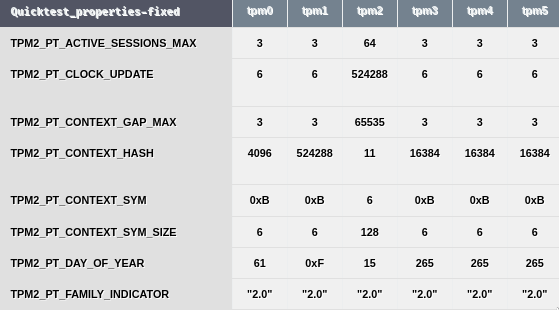
\includegraphics[width=.8\linewidth]{img/visualizations/tpm-support-properties.png}
    \caption{TPM properties}
  \end{subfigure}
  
  \begin{subfigure}{\linewidth}
    \centering
    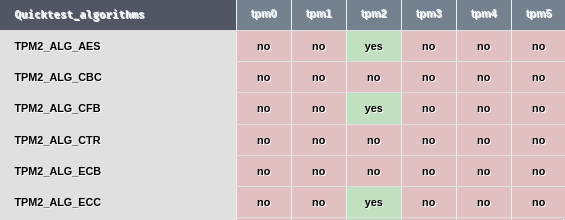
\includegraphics[width=.8\linewidth]{img/visualizations/tpm-support-algorithms.png}
    \caption{TPM algorithms}
  \end{subfigure}  

  \begin{subfigure}{\linewidth}
    \centering
    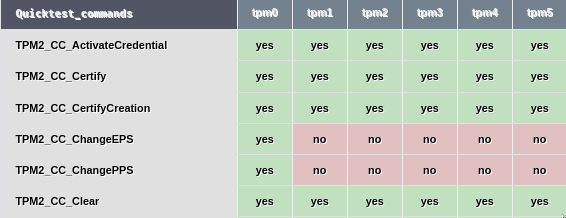
\includegraphics[width=.8\linewidth]{img/visualizations/tpm-support-commands.png}
    \caption{TPM commands}
  \end{subfigure}  
  \caption{Parts of TPM support table}  
\end{figure} 

\begin{landscape}
    \begin{figure}[!t]
        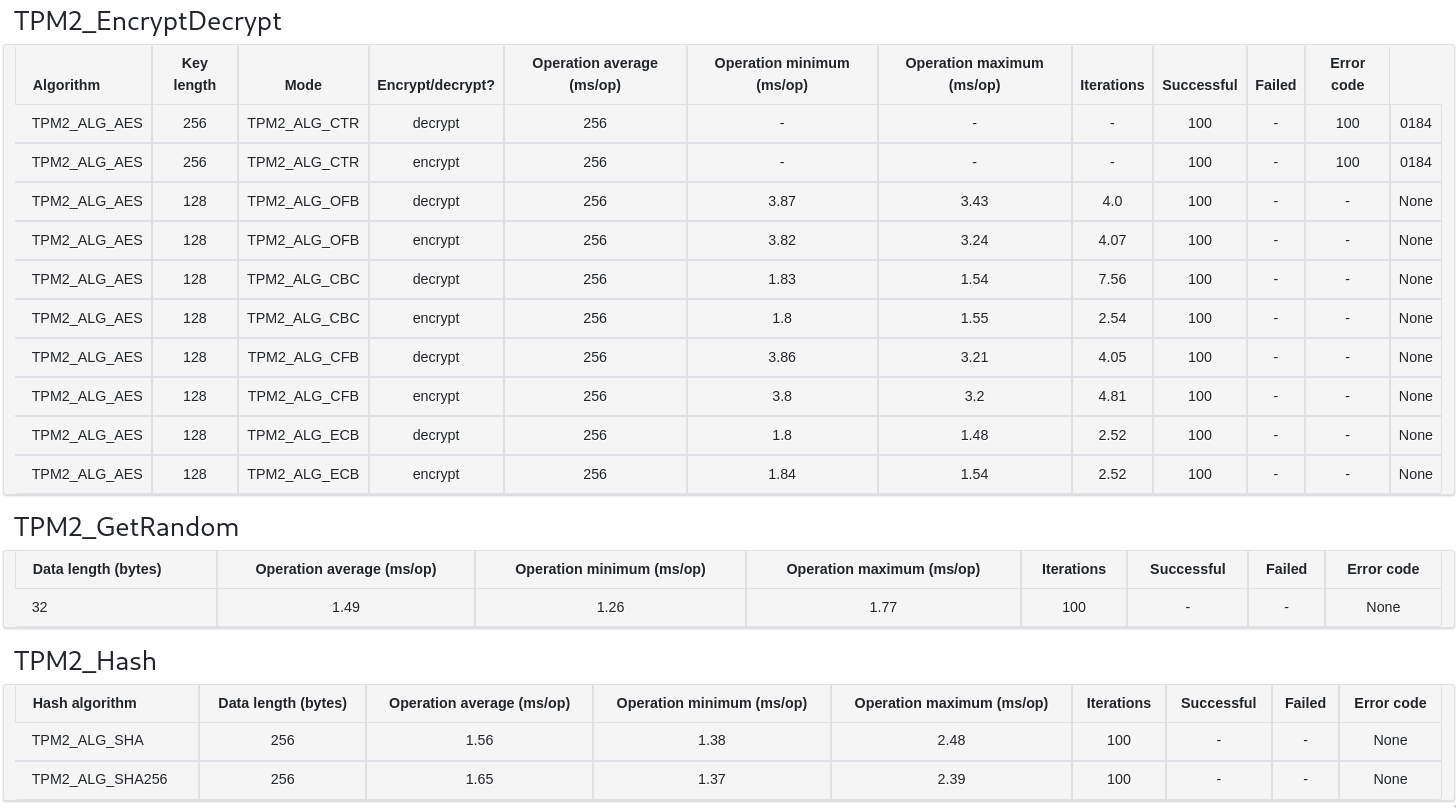
\includegraphics[width=\linewidth, height=\textwidth]{img/visualizations/tpm-execution-time.png}
        \caption{A part of Execution time visualization for INTC Intel 401.1.0.0}
    \end{figure}
\end{landscape}

\begin{landscape}
    \begin{figure}[!t]
        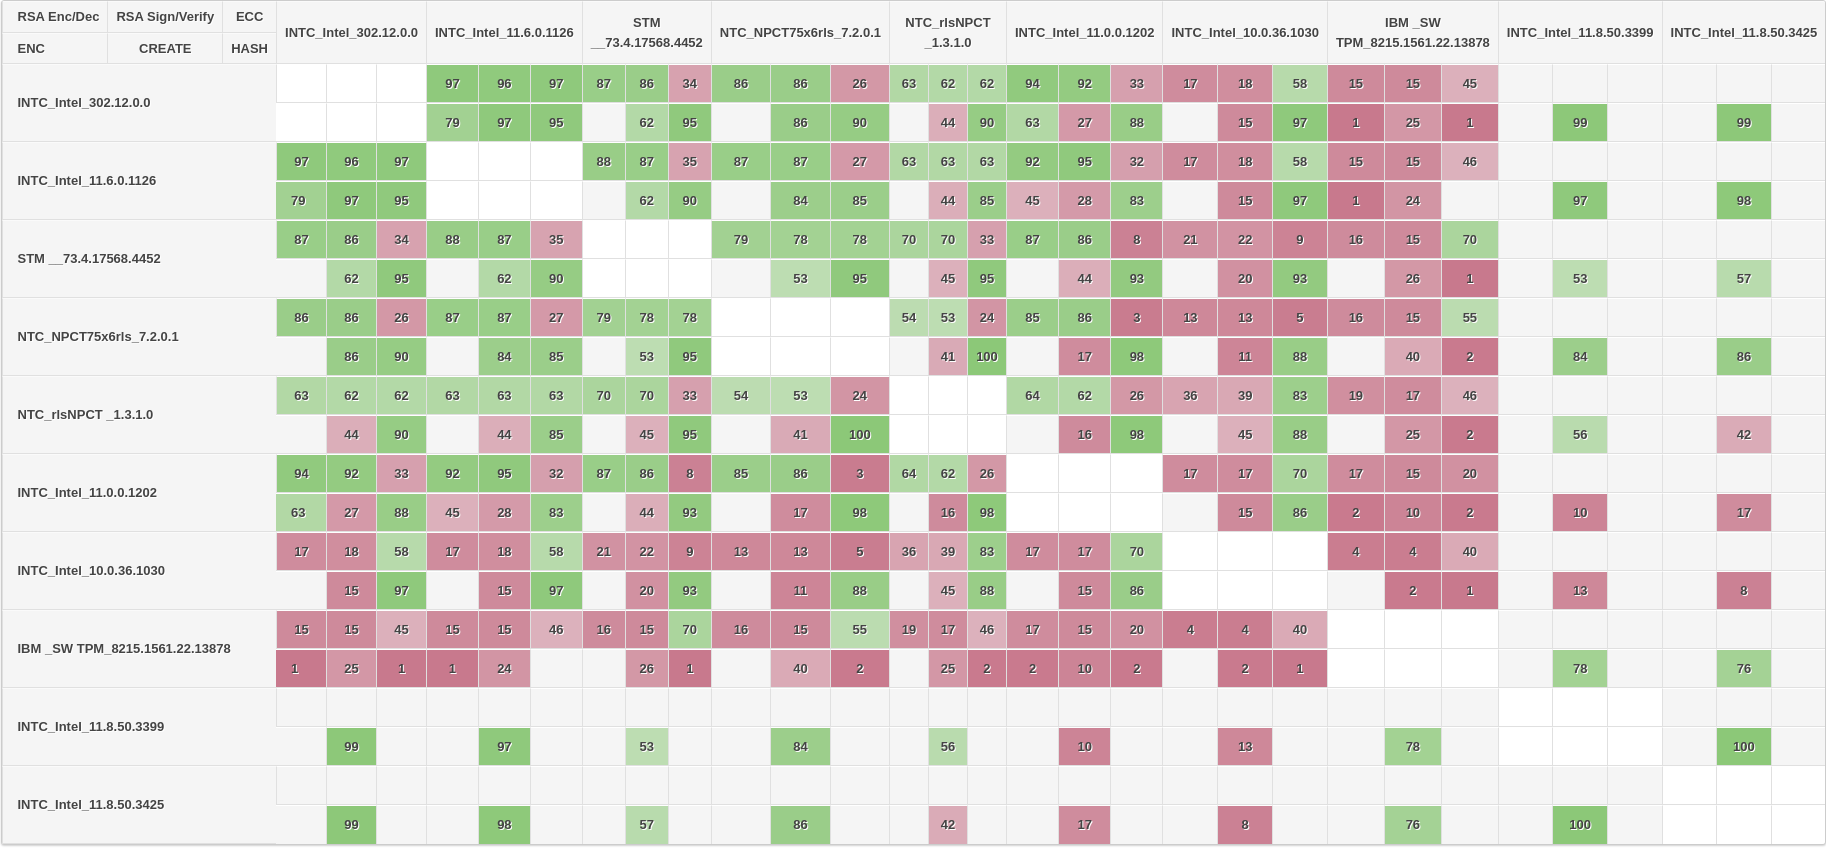
\includegraphics[width=\linewidth, height=\textwidth]{img/visualizations/tpm-similarity.png}
        \caption{A similarity table for TPMs. The table shows only a subset of visualized TPMs.}
    \end{figure}
\end{landscape}

\begin{landscape}
\begin{figure}[!t]
    \centering
    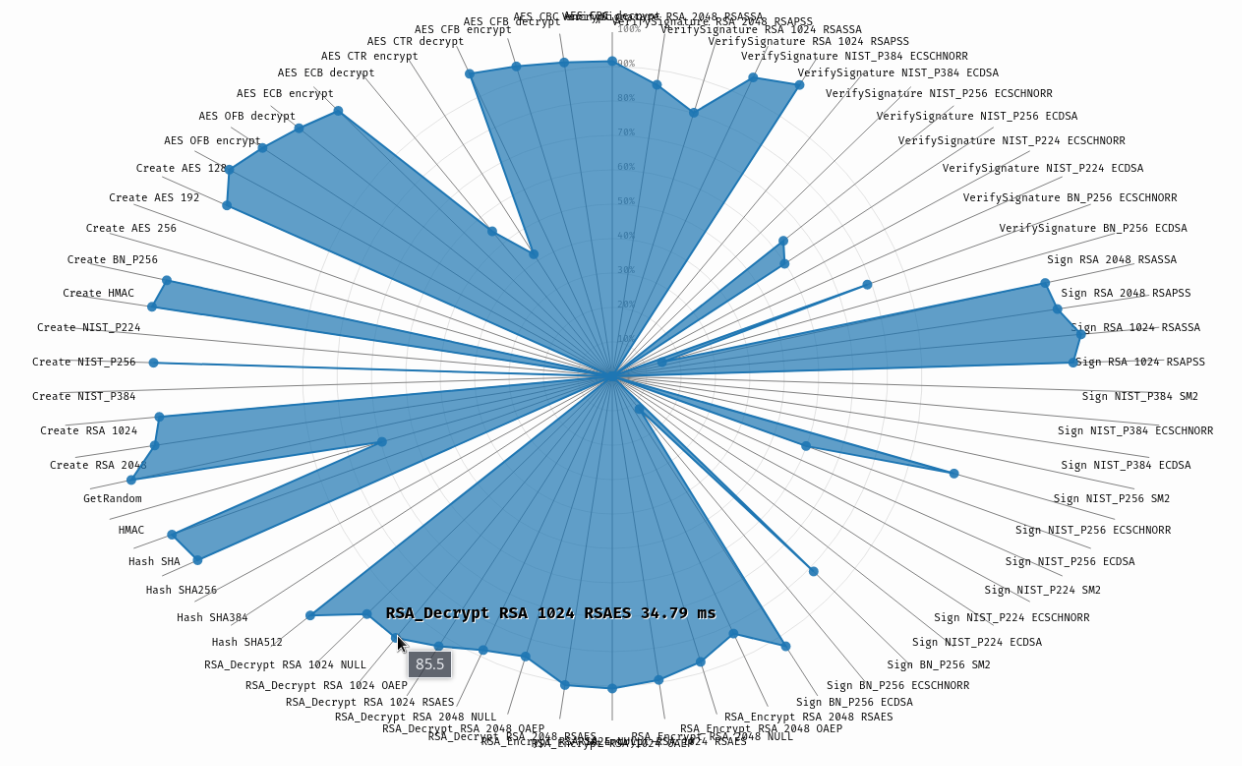
\includegraphics[width=\linewidth]{img/visualizations/INTC_Intel_302.12.0.0 radar graph.png}
    \caption{
    The radar graph of the INTC Intel 302.12.0.0 TPM.
    }
\end{figure}
\end{landscape}

\begin{landscape}
\begin{figure}[!t]
    \centering
    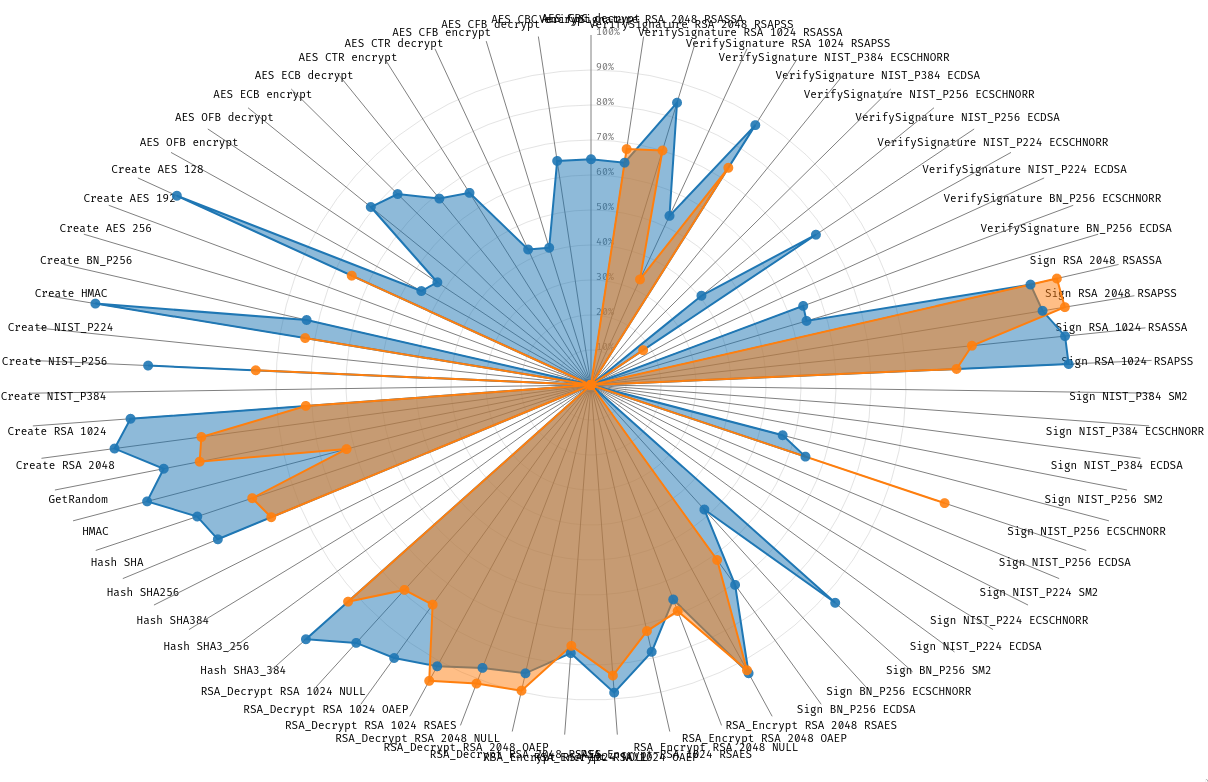
\includegraphics[width=\linewidth]{img/visualizations/INTC_Intel_11.5.0.1058_vs_IFX_SLB9670_7.63.13.6400-radar-comparison.png}
    \caption{
    Comparison radar graph between INTC Intel 11.5.0.1058 and IFX SLB9670 7.63.13.6400.
    }
\end{figure}
\end{landscape}

\begin{figure}[H]
    \centering
    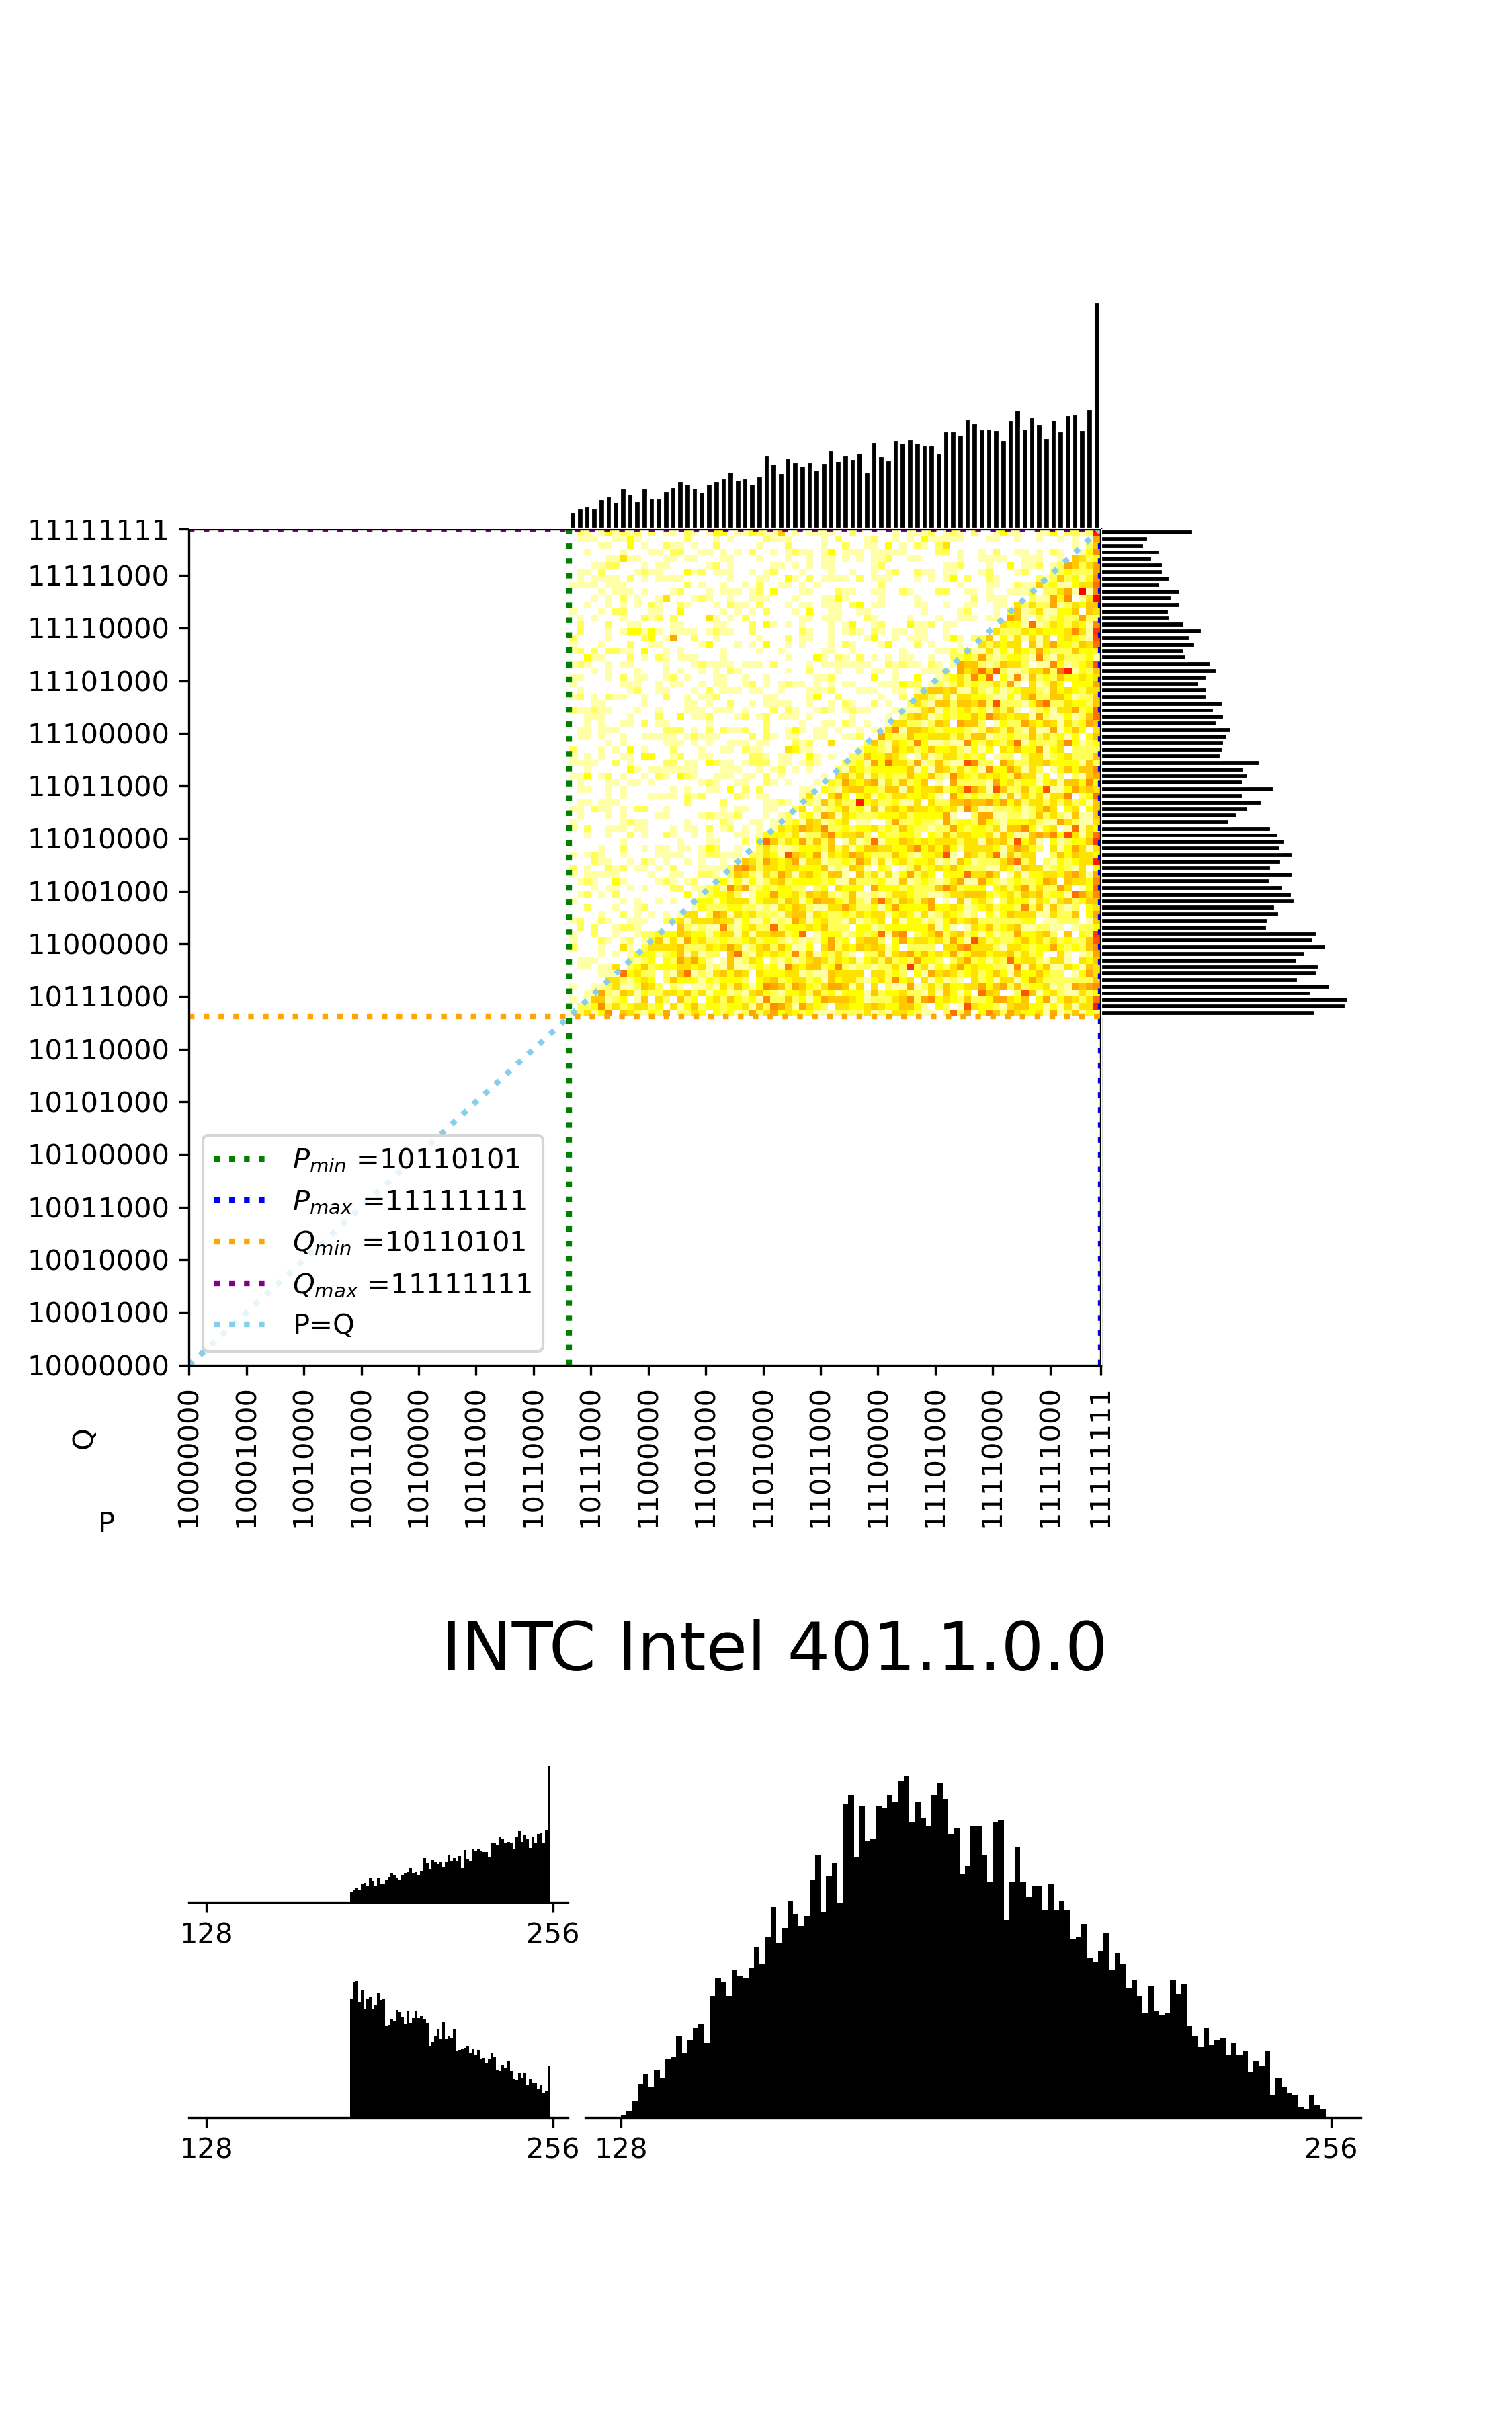
\includegraphics[width=\textwidth,height=\textheight-1.5cm, keepaspectratio]{img/visualizations/rsa.png}
    \caption{TPM heatmap of MSB values for 10000 RSA 1024-bit key pairs}
    \label{fig:heatmap-rsa-10000-1024}
\end{figure}

\begin{figure}[H]
    \centering
    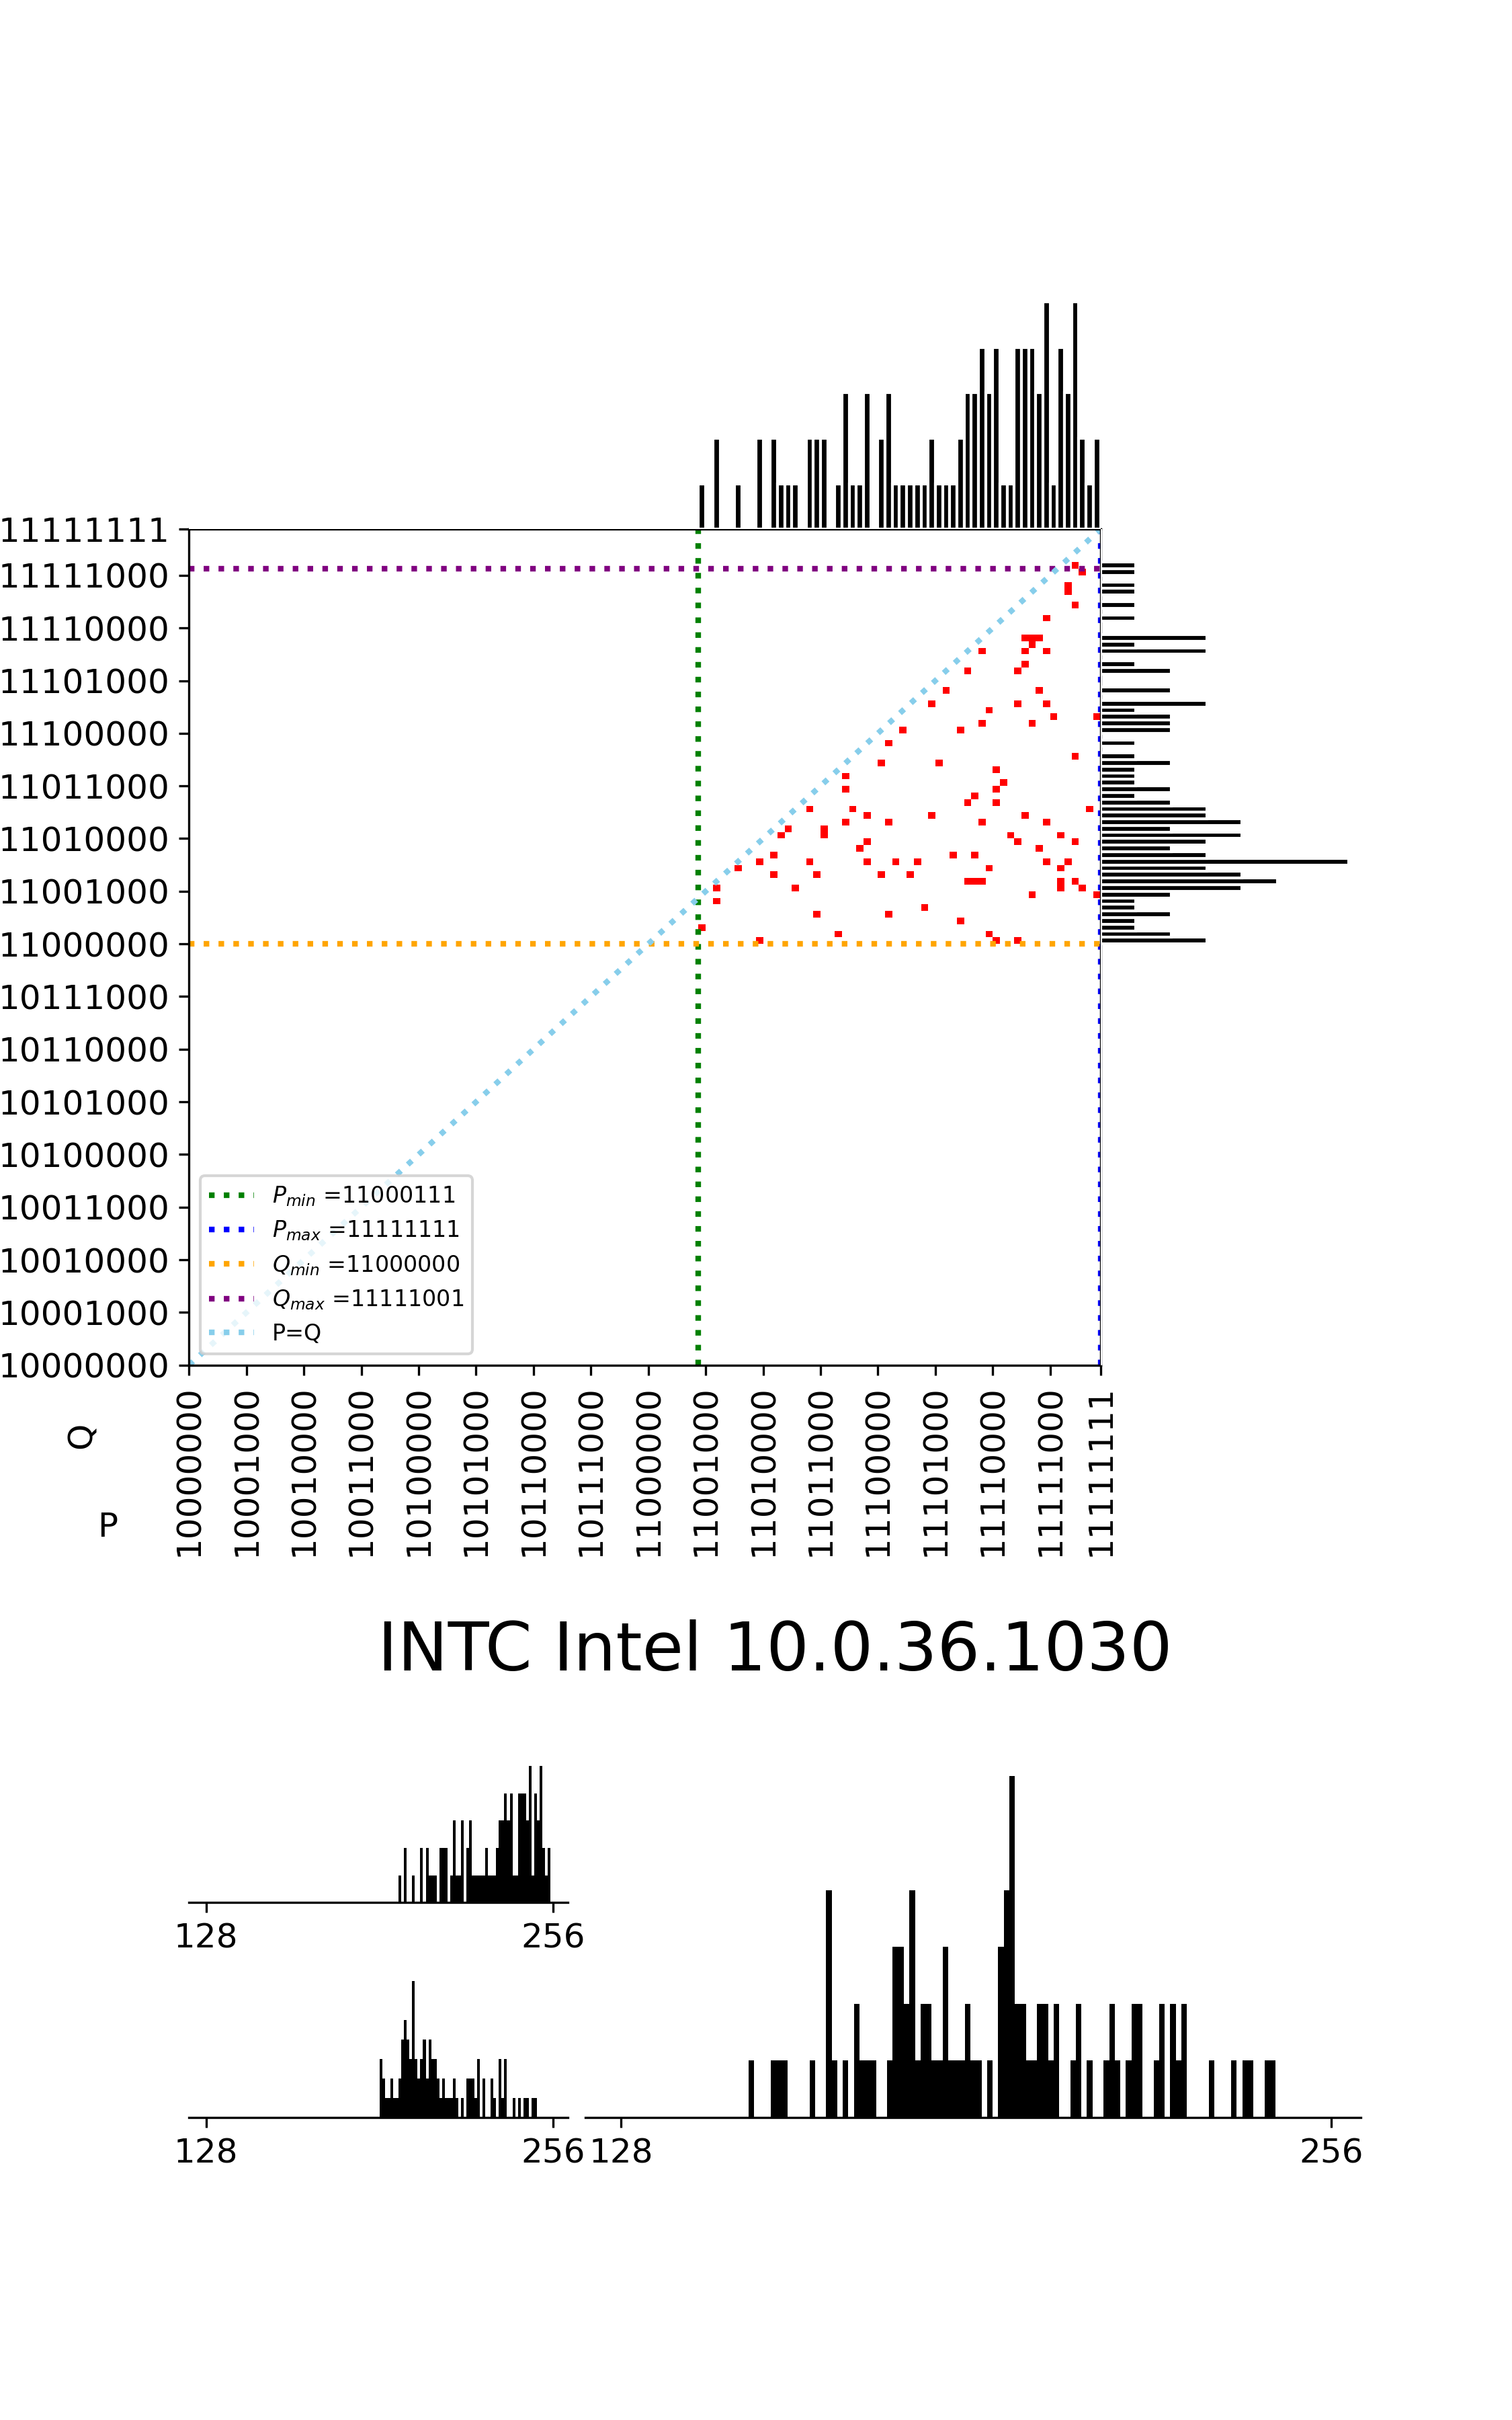
\includegraphics[width=\textwidth,height=\textheight-1.5cm, keepaspectratio]{img/visualizations/rsa1.png}
    \caption{TPM heatmap of MSB values for 100 RSA 2048-bit key pairs}
    \label{fig:heatmap-rsa-100-2048}
\end{figure}

\begin{figure}[H]
    \centering
    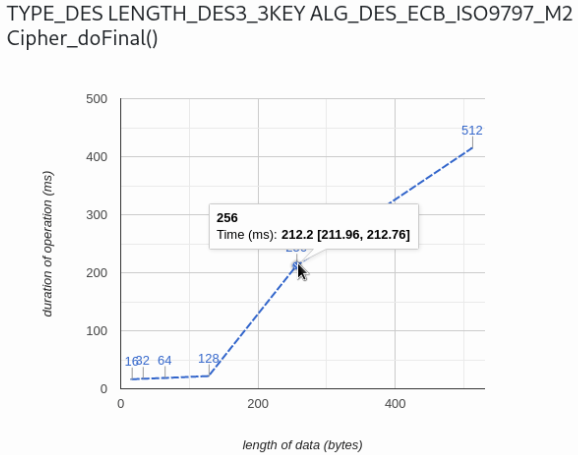
\includegraphics[width=\textwidth]{img/visualizations/NXP J3A080-scalability-DES3.png}
    \caption{NXP J30808 JavaCard smart card scalability chart}
\end{figure}

\begin{figure}[H]
    \centering
    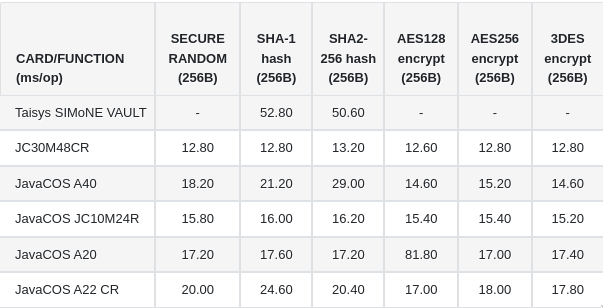
\includegraphics[width=\textwidth]{img/visualizations/jc-comparative-table.png}
    \caption{A part of the comparative table for JavaCard smart cards}
    \label{fig:my_label}
\end{figure}


\renewcommand{\thechapter}{C}
\chapter{Diagram and Dataset examples}\label{appendix:diagram-profiles}
\begin{figure}[H]
    \centering
    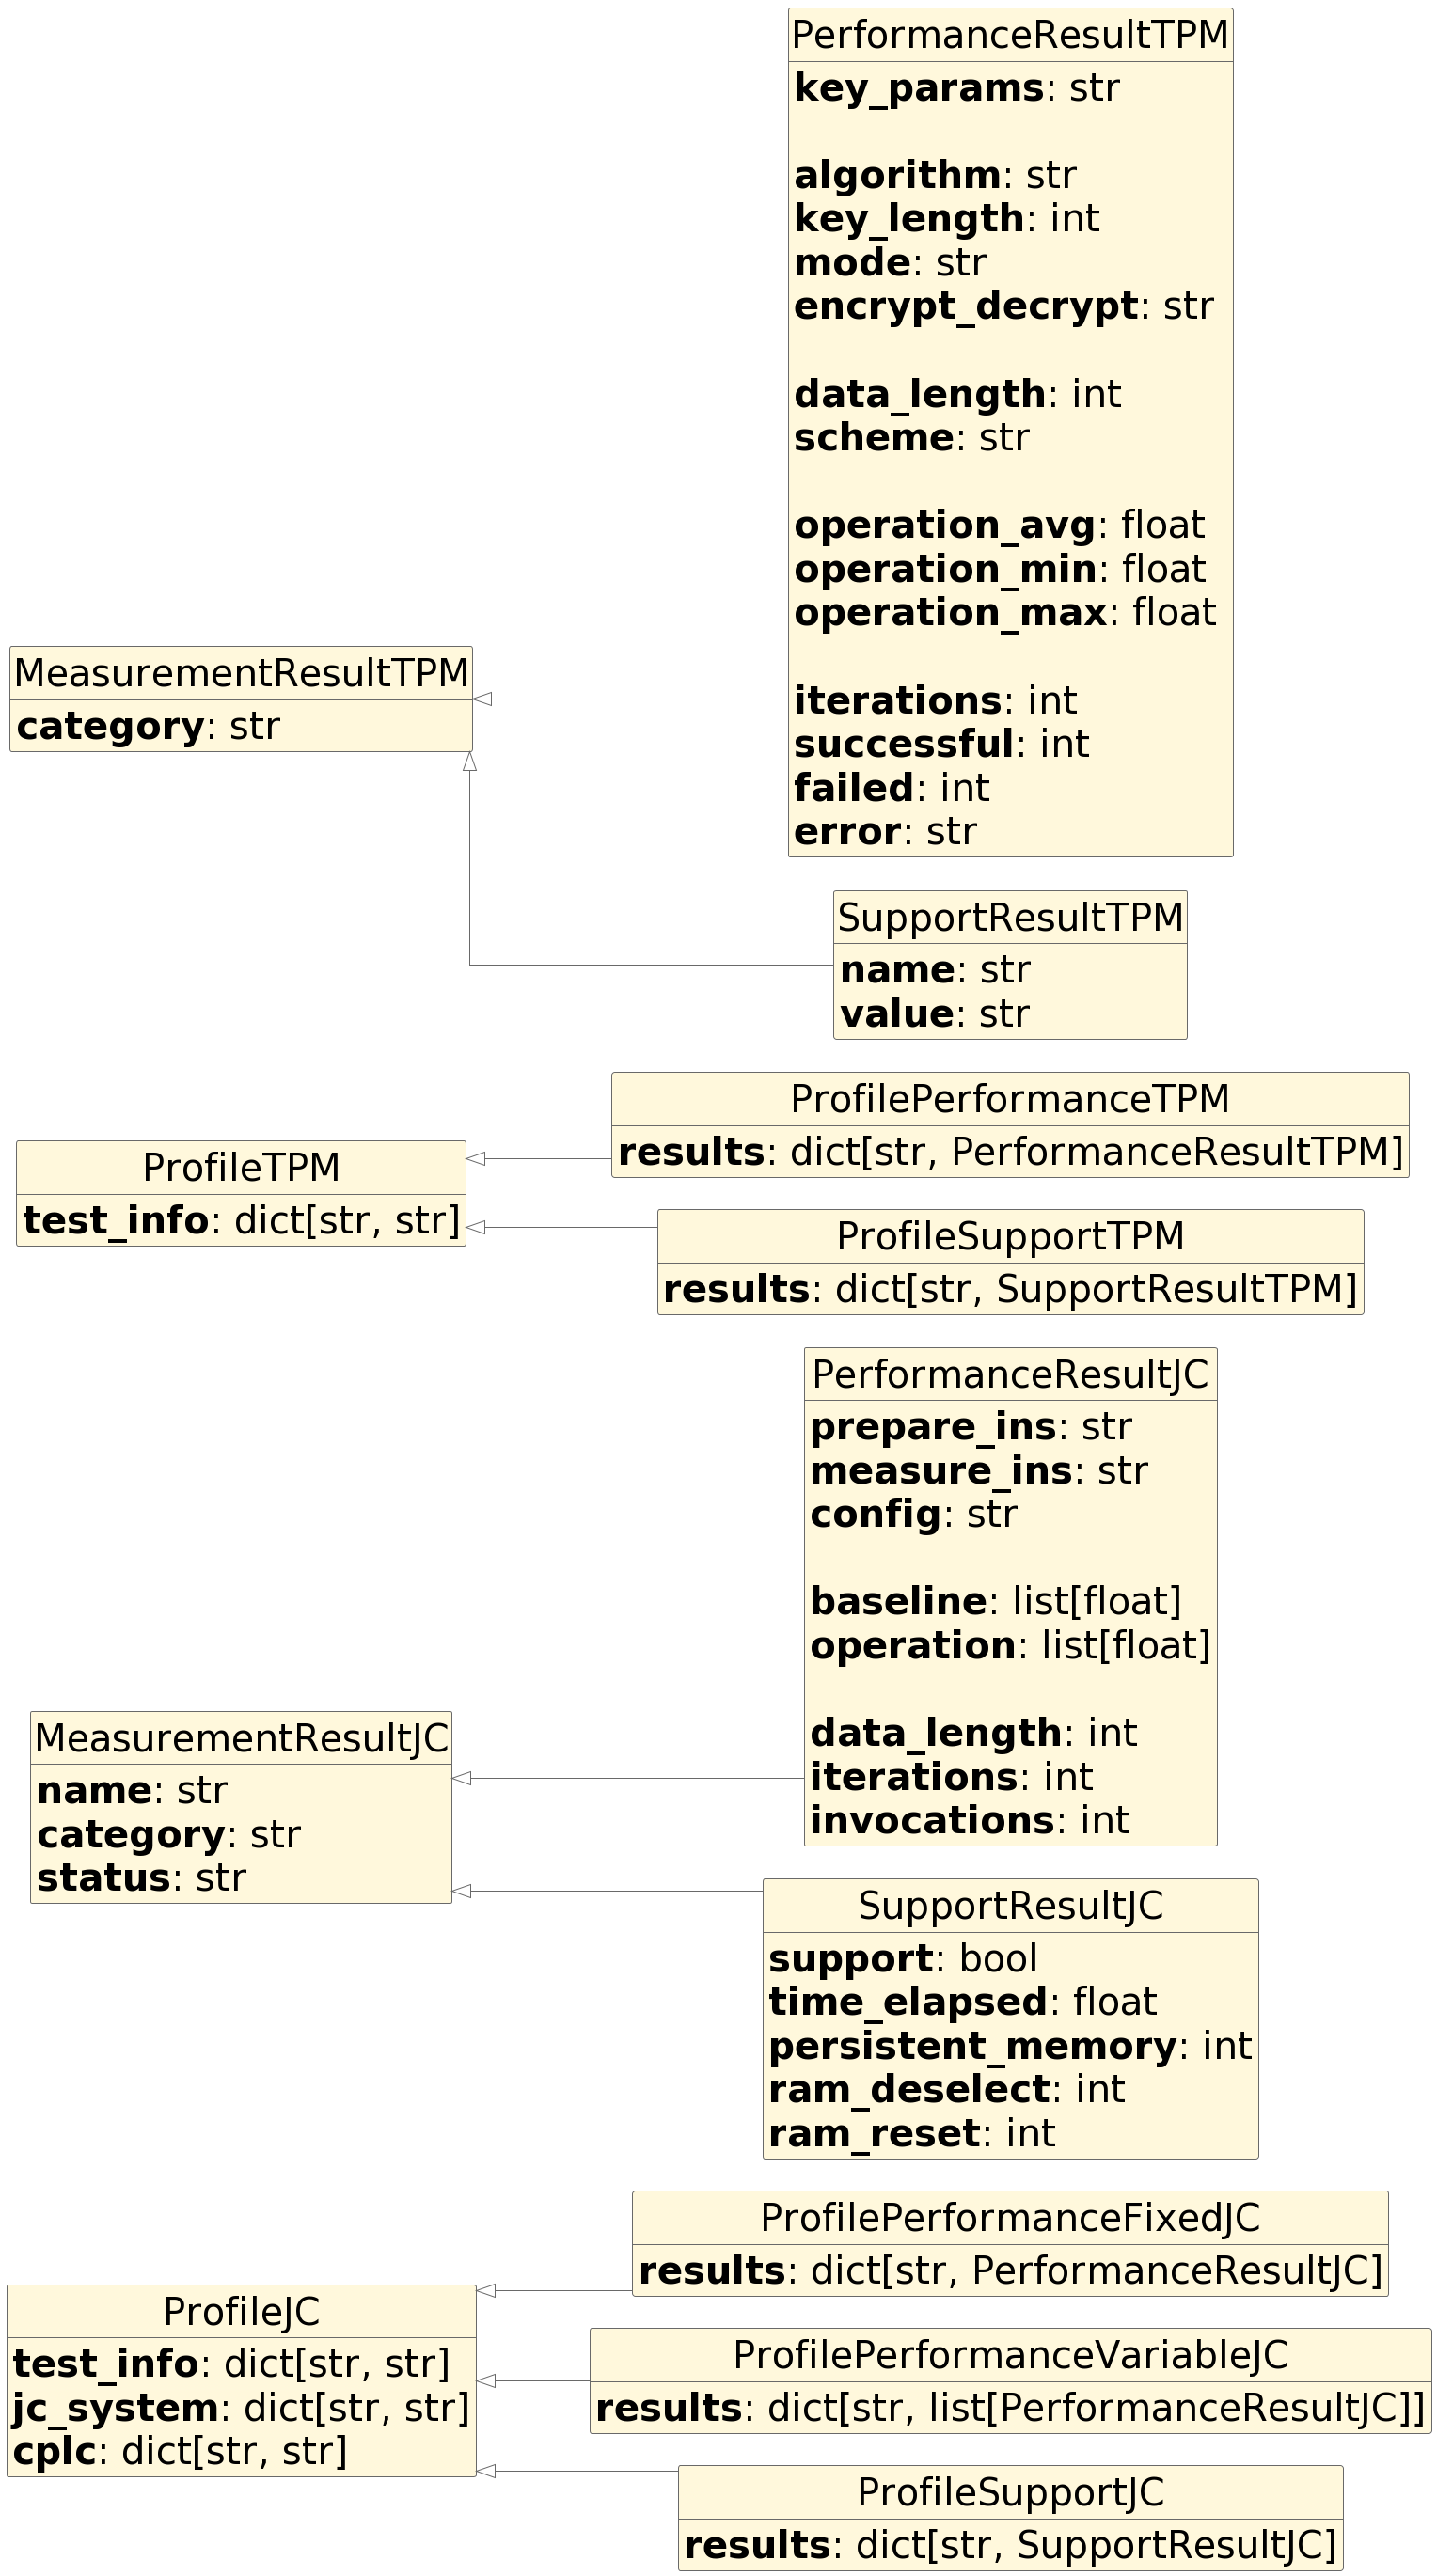
\includegraphics[width=\textwidth,height=\textheight-6cm, keepaspectratio]{img/diagrams/object_diagram.png}
    \caption{Diagram of Performance and Support device profiles for TPMs and JavaCards.}
    \label{fig:dev-profiles-diagram}
\end{figure}


\begin{figure}
    \centering
    \lstinputlisting[]{img/datasets/tpm-perf/tpm-perf.csv}
    \caption{A part of the performance device profile for TPMs. The initial information in the upper part of the figure corresponds to \texttt{test\_info} attribute of \texttt{ProfileTPM} class, whereas the rest of the figure shows TPM performance results corresponding to \texttt{PerformanceResultTPM} class. Both of the mentioned classes could be seen in \myref{Figure}{fig:dev-profiles-diagram}. Ellipses mean skipped lines and are not a part of any device profiles.}
\end{figure}

\begin{figure}
    \centering
    \lstinputlisting[]{img/datasets/tpm-support/tpm-support.csv}
    \caption{A shortened support device profile for TPMs. Hexadecimal numbers in the lower half of the profile are identifiers of supported algorithms, commands, and curves.}
\end{figure}

\begin{figure}
    \centering
    \lstinputlisting[]{img/datasets/jc-header/jc-tinfo.csv}
    \caption{This is a common part of all device profiles for JavaCard smart cards, initial contents are very similar. All three parts correspond to attributes in \texttt{ProfileJC} class seen in \myref{Figure}{fig:dev-profiles-diagram}. First part corresponds to \texttt{test\_info} attribute, second corresponds to \texttt{jc\_system} attribute and last one corresponds to \texttt{cplc} attribute.Figure created from device profiles at \cite{jcalgtestResultsRepo}.}
\end{figure}

\begin{figure}
    \centering
    \lstinputlisting[]{img/datasets/jc-fixed/fix-results.csv}
    \caption{This corresponds to a part of the performance device profile for JavaCard smart cards where fixed data length performance was measured. Noticeably, many items in each measurement correspond to the attributes of \texttt{PerformanceResultJC} class seen in \myref{Figure}{fig:dev-profiles-diagram}. Figure created from device profiles at \cite{jcalgtestResultsRepo}.}
\end{figure}

\begin{figure}
    \centering
    \lstinputlisting[]{img/datasets/jc-variable/var-results.csv}
    \caption{This is a part of the performance device profile for JavaCard smart cards, where variable data length performance was measured. As can be seen in the upper half of the figure, some measurements could not be performed because the device does not support such algorithms. In the lower half of the figure, two successful measurements were performed for 16 and 32-byte data lengths. Figure created from device profiles at \cite{jcalgtestResultsRepo}.}
\end{figure}

\begin{figure}
    \centering
    \lstinputlisting[]{img/datasets/jc-support/jc-support.csv}
    \caption{A part of the support device profile for JavaCard smart cards. Figure created from device profiles at \cite{jcalgtestResultsRepo}.}
\end{figure}

\renewcommand{\thechapter}{D}
\chapter{Data Attachments}
\begin{itemize}
    \item \texttt{AlgTest\_pyProcess} folder containing the implementation of \texttt{AlgTest pyProcess} tool
    \item \texttt{jcalgtest\_visualizations} folder containing the JavaCard smart card visualizations generated by \texttt{AlgTest pyProcess} tool. Stylesheets and JavaScript is provided in \texttt{assets} folder and some decorative images are provided in \texttt{pics} folder. Decorative images were taken from \texttt{crocs-muni/jcalgtest\_results} on GitHub.
    
    \item \texttt{tpmalgtest\_visualizations} folder containing the TPM visualizations generated by \texttt{AlgTest pyProcess} tool. Stylesheets and JavaScript is provided in \texttt{assets} folder 
\end{itemize}
